\documentclass[12pt]{beamer}
\usepackage{beamerthemeHannover, graphicx, clrscode, amsmath, amssymb, multicol}
\usepackage{textcomp} \usepackage{verbatim}
\usepackage{listings}
\setbeamercolor{sidebar}{use=structure,bg=green!20!blue!30}

\title{Crafting Type: What Software Freedom Means To Me}
\author[@dukeleto]{Jonathan "Duke" Leto}
\date{}

\begin{document}

\frame{
    \titlepage
    \begin{center}
%    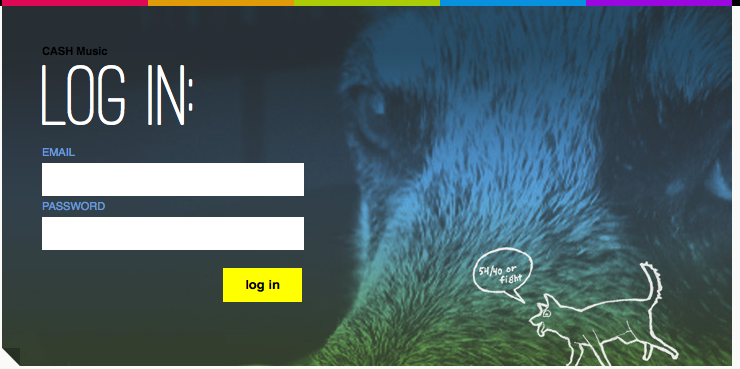
\includegraphics[scale=0.3]{cm.png}
    \end{center}
}

\frame{
    \frametitle{What is Software Freedom?}

    Everyone should have the freedom to look at, distribute and modify (if they want) software.
}

\frame{
    \frametitle{What is Software Freedom?}

    A "commons", where anybody with an Internet connection has the freedom to  access and contribute to free software.
}

\frame{
    \frametitle{What is Software Freedom?}

    Every time somebody write Free Software, everybody in the world benefits from it. No one is excluded.
}

\frame{
    \frametitle{What is the opposite of Software Freedom?}

    Software Oppression
    \begin{itemize}
        \item Blocking communication
        \item i.e. Preventing knowledge transfer for finanical/power gain
        \item Propaganda
        \item Orwellian Augmented Reality
    \end{itemize}
}

\frame{
    \frametitle{What is the difference between Free and Open?}

    Open = derivative works can be proprietary/commercial \\
    Free = "viral" openness + freedom

}

\frame{
    \frametitle{Why Should I Care?}

    Everybody benefits from free and open code and data. \\
    Only a select few people benefit from proprietary code or data.
}


\frame{
    \frametitle{Interesting Projects}
    \begin{itemize}
        \item FontForge
        \item Font Awesome - Iconic font
        \item Twitter Bootstrap - Mobile friendly website by default
    \end{itemize}
}


\frame{
    \frametitle{ Find Me }
    \begin{center}
        \begin{itemize}
           \item duke@leto.net
           \item @dukeleto
           \item http://leto.github.com
           \item http://linkedin.leto.net
        \end{itemize}
    \end{center}
}
\end{document}
